Supppose we are given
%\begin{multicols}{2}
\begin{itemize}
	\item binary columns $\bit{1}$, $\bit{2}$, $\bit{3}$ and $\bit{4}$,
	\item counter-constant columns  \sourceOne{}, \sourceTwo{}, \target{},
	\item byte columns \sourceOne{}\byte{} and \sourceTwo{}\byte{},
	\item counter-constant columns \sourceOne{}\mark{} and \size{},
	\item accumulator columns \acc{1} and \acc{2},
	\item two columns \col{P1} and \col{P2},
	\item a ``counter column'' \ct{}.
	%\item[\vspace{\fill}]
\end{itemize}
%\end{multicols}
The interpreation is as follows:
\sourceOne{} contains a limb from which we extract a suffix;
\acc{1} will accumulate the bytes of said suffix;
\sourceTwo{} contains a limb from which we extract a prefix;
\acc{2} will accumulate the bytes of said prefix;
\sourceOne{}\byte{} and \sourceTwo{}\byte{} are the respective byte decompositions;
\sourceOne{}\mark{} is the offset within \sourceOne{} from where we start harvesting bytes;
\size{} is the total number of bytes to harvest;
\target{} will be made to contain the prefix extracted from \sourceOne{} followed by the prefix extracted from \sourceTwo{} (left aligned);
the assumption is that $\sourceOne{}\mark{} + \size{} > \llarge$ so that two byte sources are required to build \target{};
$\bit{1}$ plateaus at \sourceOne{}\mark{};
$\bit{2}$ plateaus at $\sourceOne{}\mark{} + \size{} - \llarge$;
$\bit{3}$ plateaus at $\llarge - \sourceOne{}\mark{}$;
$\bit{4}$ plateaus at $\size{}$;
$\col{P1}$ and $\col{P2}$ are ``powers of 256'' columns with $\col{P1}$ pegged to $\bit{3}$ and $\col{P2}$ pegged to $\bit{4}$;
together they build the correct powers of 256 required for shifting the extracted prefix and suffix and building \target{}. Compare with figure~\ref{fig: two to one padded}.

The following collection of constraints ensures the desired behaviour:
\begin{enumerate}
	\item binary plateau constraints:
	\begin{enumerate}
		\item $\plateau(\bit{1}, \sourceOne{}\mark{}; \ct{})$,
		\item $\plateau(\bit{2}, \sourceOne{}\mark{} + \size{} - \llarge; \ct{})$,
		\item $\plateau(\bit{3}, \llarge - \sourceOne{}\mark{}; \ct{})$;
		\item $\plateau(\bit{4}, \size{}; \ct{})$;
	\end{enumerate}
	\item prefix and suffix constraints:
	\begin{enumerate}
		\item  $\compSuffix(\acc{1}, \sourceOne{}\byte{}, \bit{1}; \ct{})$;
		\item  $\compPrefix(\acc{2}, \sourceTwo{}\byte{}, \bit{2}; \ct{})$;
	\end{enumerate}
	\item power constraints: 
	\begin{enumerate}
		\item $\power(\col{P1}, \bit{3}; \ct{})$;
		\item $\power(\col{P2}, \bit{4}; \ct{})$;
	\end{enumerate}
	\item value enforcement
	\[
		\If\ct{}_{i} = \llargeMO~
		\Then
		\target{}_{i}
		=
		\acc{1}_{i}\cdot \col{P1}_{i}
		+
		\acc{2}_{i}\cdot \col{P2}_{i}.
	\]
\end{enumerate}
We use the short hand 
\[
	\twoToOnePadded
	\left(
	\begin{array}{c}
	\sourceOne{}, \sourceTwo{}, \target{}; \sourceOne{}\byte{}, \sourceTwo{}\byte{};\\
	\acc{1}, \acc{2}; \col{P1}, \col{P2};\\
	\sourceOne{}\mark{}, \size{}; \bit{1}, \bit{2}, \bit{3}, \bit{4}; \ct{};
	\end{array}
	\right)
\]

\begin{figure}[h!]
\centering
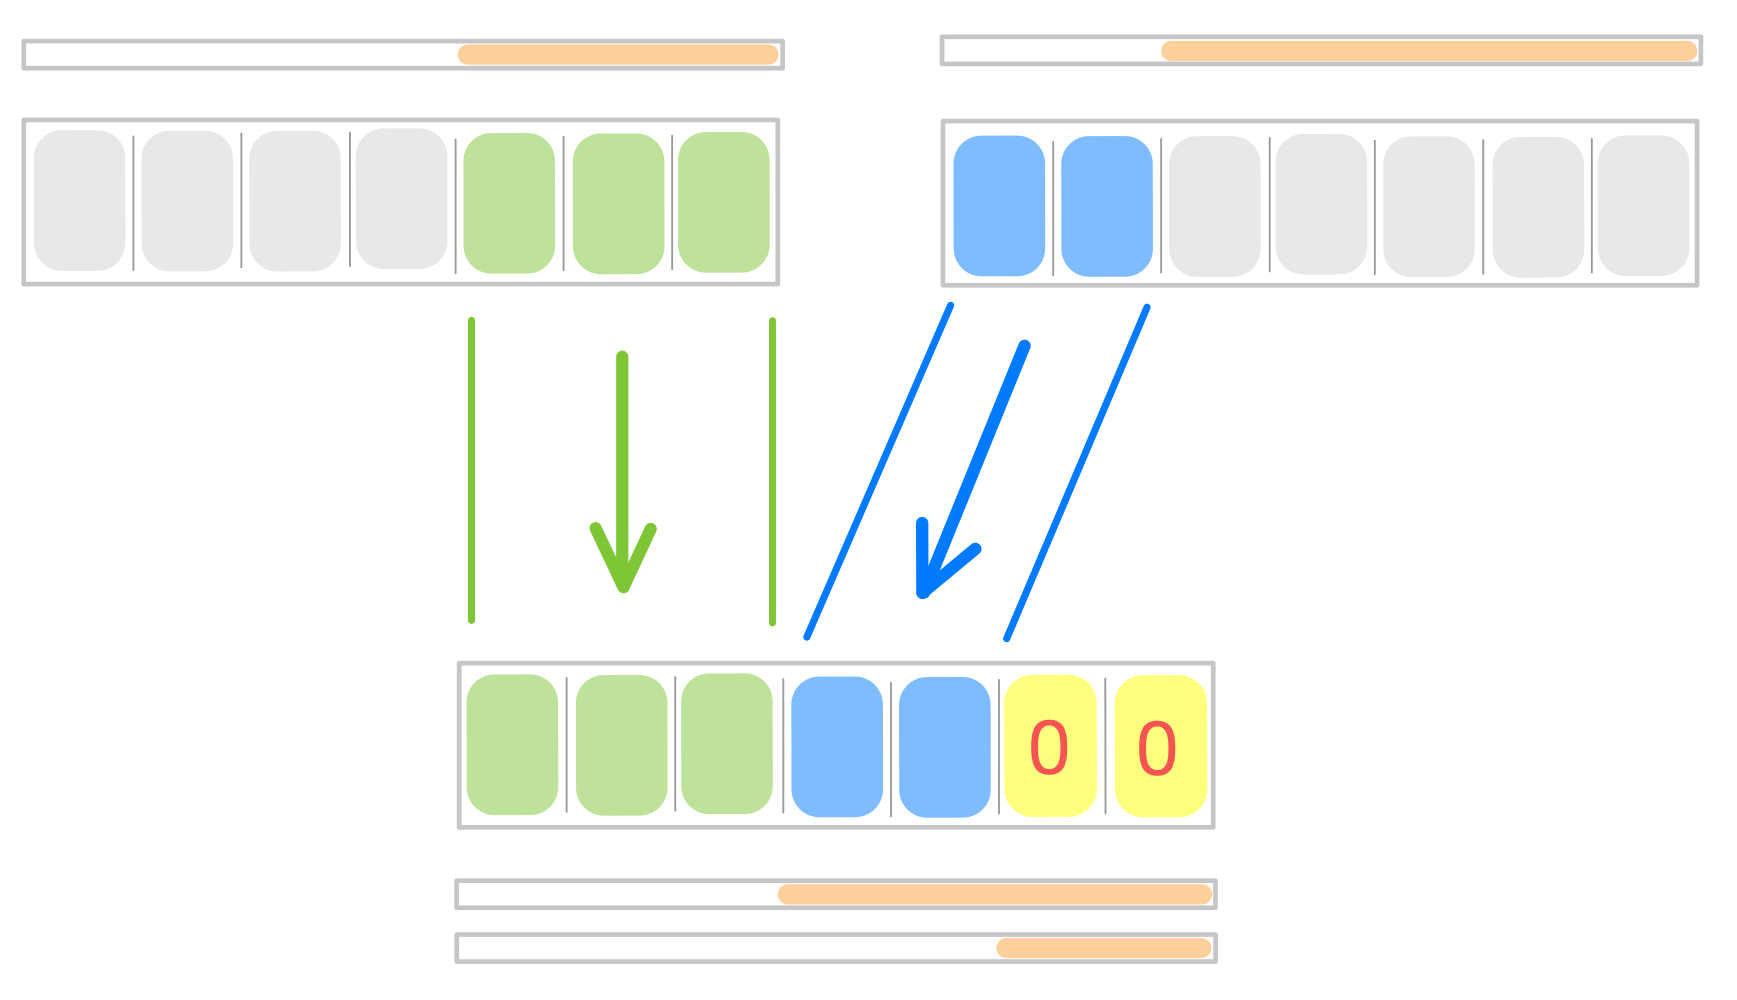
\includegraphics[width = 0.5\textwidth]{drawing/2_to_1_padded}
\label{fig: two to one padded}
\caption{Representation of the constraints implemented by $\twoToOnePadded$.}
\end{figure}